\documentclass[brazil,times]{abnt}
\usepackage[T1]{fontenc}
\usepackage[utf8]{inputenc}
\usepackage{url}
\usepackage{graphicx}
%\usepackage{hyperref} 

\makeatletter
\usepackage{babel}
\makeatother
\begin{document}

\autor{Pedro Paulo Vezzá Campos}

\titulo{A história e evolução dos sistemas e redes de computadores}

\comentario{Trabalho apresentado para avaliação na disciplina INE5414, do
curso de Bacharelado em Ciências da Computação, turma 04208, da Universidade   
Federal de Santa Catarina, ministrada pelo professor Carlos Becker Westphall}

\instituicao{Departamento de Informática e Estatística \par Centro
Tecnológico \par Universidade Federal de Santa Catarina}

\local{Santa Catarina - SC, Brasil}

\data{13 de agosto de 2010}

\capa

\folhaderosto

\tableofcontents
% \chapter{Introdução\label{cap:introducao}}
% Com o intuito de de fornecer uma fundamentação para o estudo das redes de
% computadores, este trabalho apresenta um resumo da história e evolução dos
% sistemas computacionais e das redes de computadores, desde os primórdios até a
% atualidade.

\chapter{História da computação}
\section{Pré-História e Antiguidade}
Apesar de a Computação enquanto ciência ter sido melhor sistematizada apenas
em 1985 \cite{computing-as-discipline}, a computação começou na pré-história. O
Osso Ishango data de 20.000 AC e já apresentava indícios do uso de riscos para efetuar operações
aritméticas. \cite{osso-ishango}

\begin{figure}[htp]
\begin{center}
  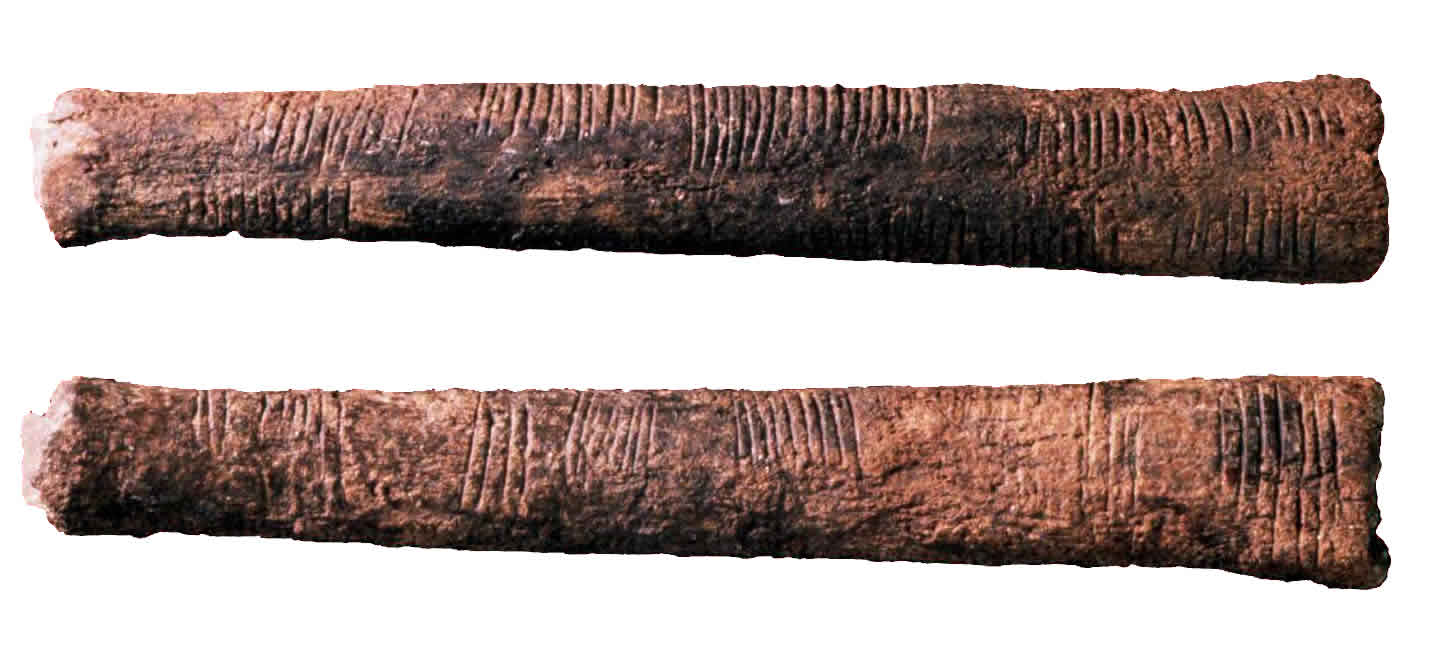
\includegraphics[width=100mm]{imagens/Ishango_bone.jpg}
  \caption[Osso Ishango, cortesia Wikipédia]{Osso Ishango, cortesia Wikipédia}
  \label{fig:osso-ishango}
\end{center}
\end{figure}

Já em 3500 AC, os Babilônios inventaram o ábaco, uma ferramenta que facilitou o
trabalho com operações matemáticas, perdurando até os dias atuais graças à sua
simplicidade e facilidade de uso. Posteriormente, em 500 AC aproximadamente, os
hindus inventaram a noção do zero, o que possibilitou a
aritimética decimal em papel.

Já no século III AC, Pingala, matemático indiano, inventou o sistema de
numeração binário. Seu trabalho ainda é aproveitado em qualquer máquina digital
atual pois a simplicidade do uso de apenas dois símbolos, 0 ou 1, ligado ou
desligado, verdadeiro ou falso, simplifica o projeto e funcionamento dos
equipamentos.

Por volta de 825, Al-Khwarizmi, matemático persa, escreveu ``Calculando com
numerais hindus'', que apresentava novos conceitos para definir
sequências de passos para completar tarefas, os algoritmos.

\section{Da Idade Moderna até 1900}
Na idade moderna houve o surgimento das primeiras máquinas calculadoras
mecânicas, como a calculadora de Pascal, e posteriormente, o projeto do
Calculador Analítico, invenção de Charles Babbage. Essa máquina possui relevante
importância histórica pois:

\begin{citacao}
O projeto, totalmente mecânico, era composto de uma memória, um engenho central,
engrenagens e alavancas usadas para a transferência de dados da memória para o
engenho central e dispositivos para entrada e saída de dados. O calculador
utilizaria cartões perfurados e seria automático.

\cite{babbage-e-ada}
\end{citacao}

%\usepackage{graphics} is needed for \includegraphics
\begin{figure}[htp]
\begin{center}
  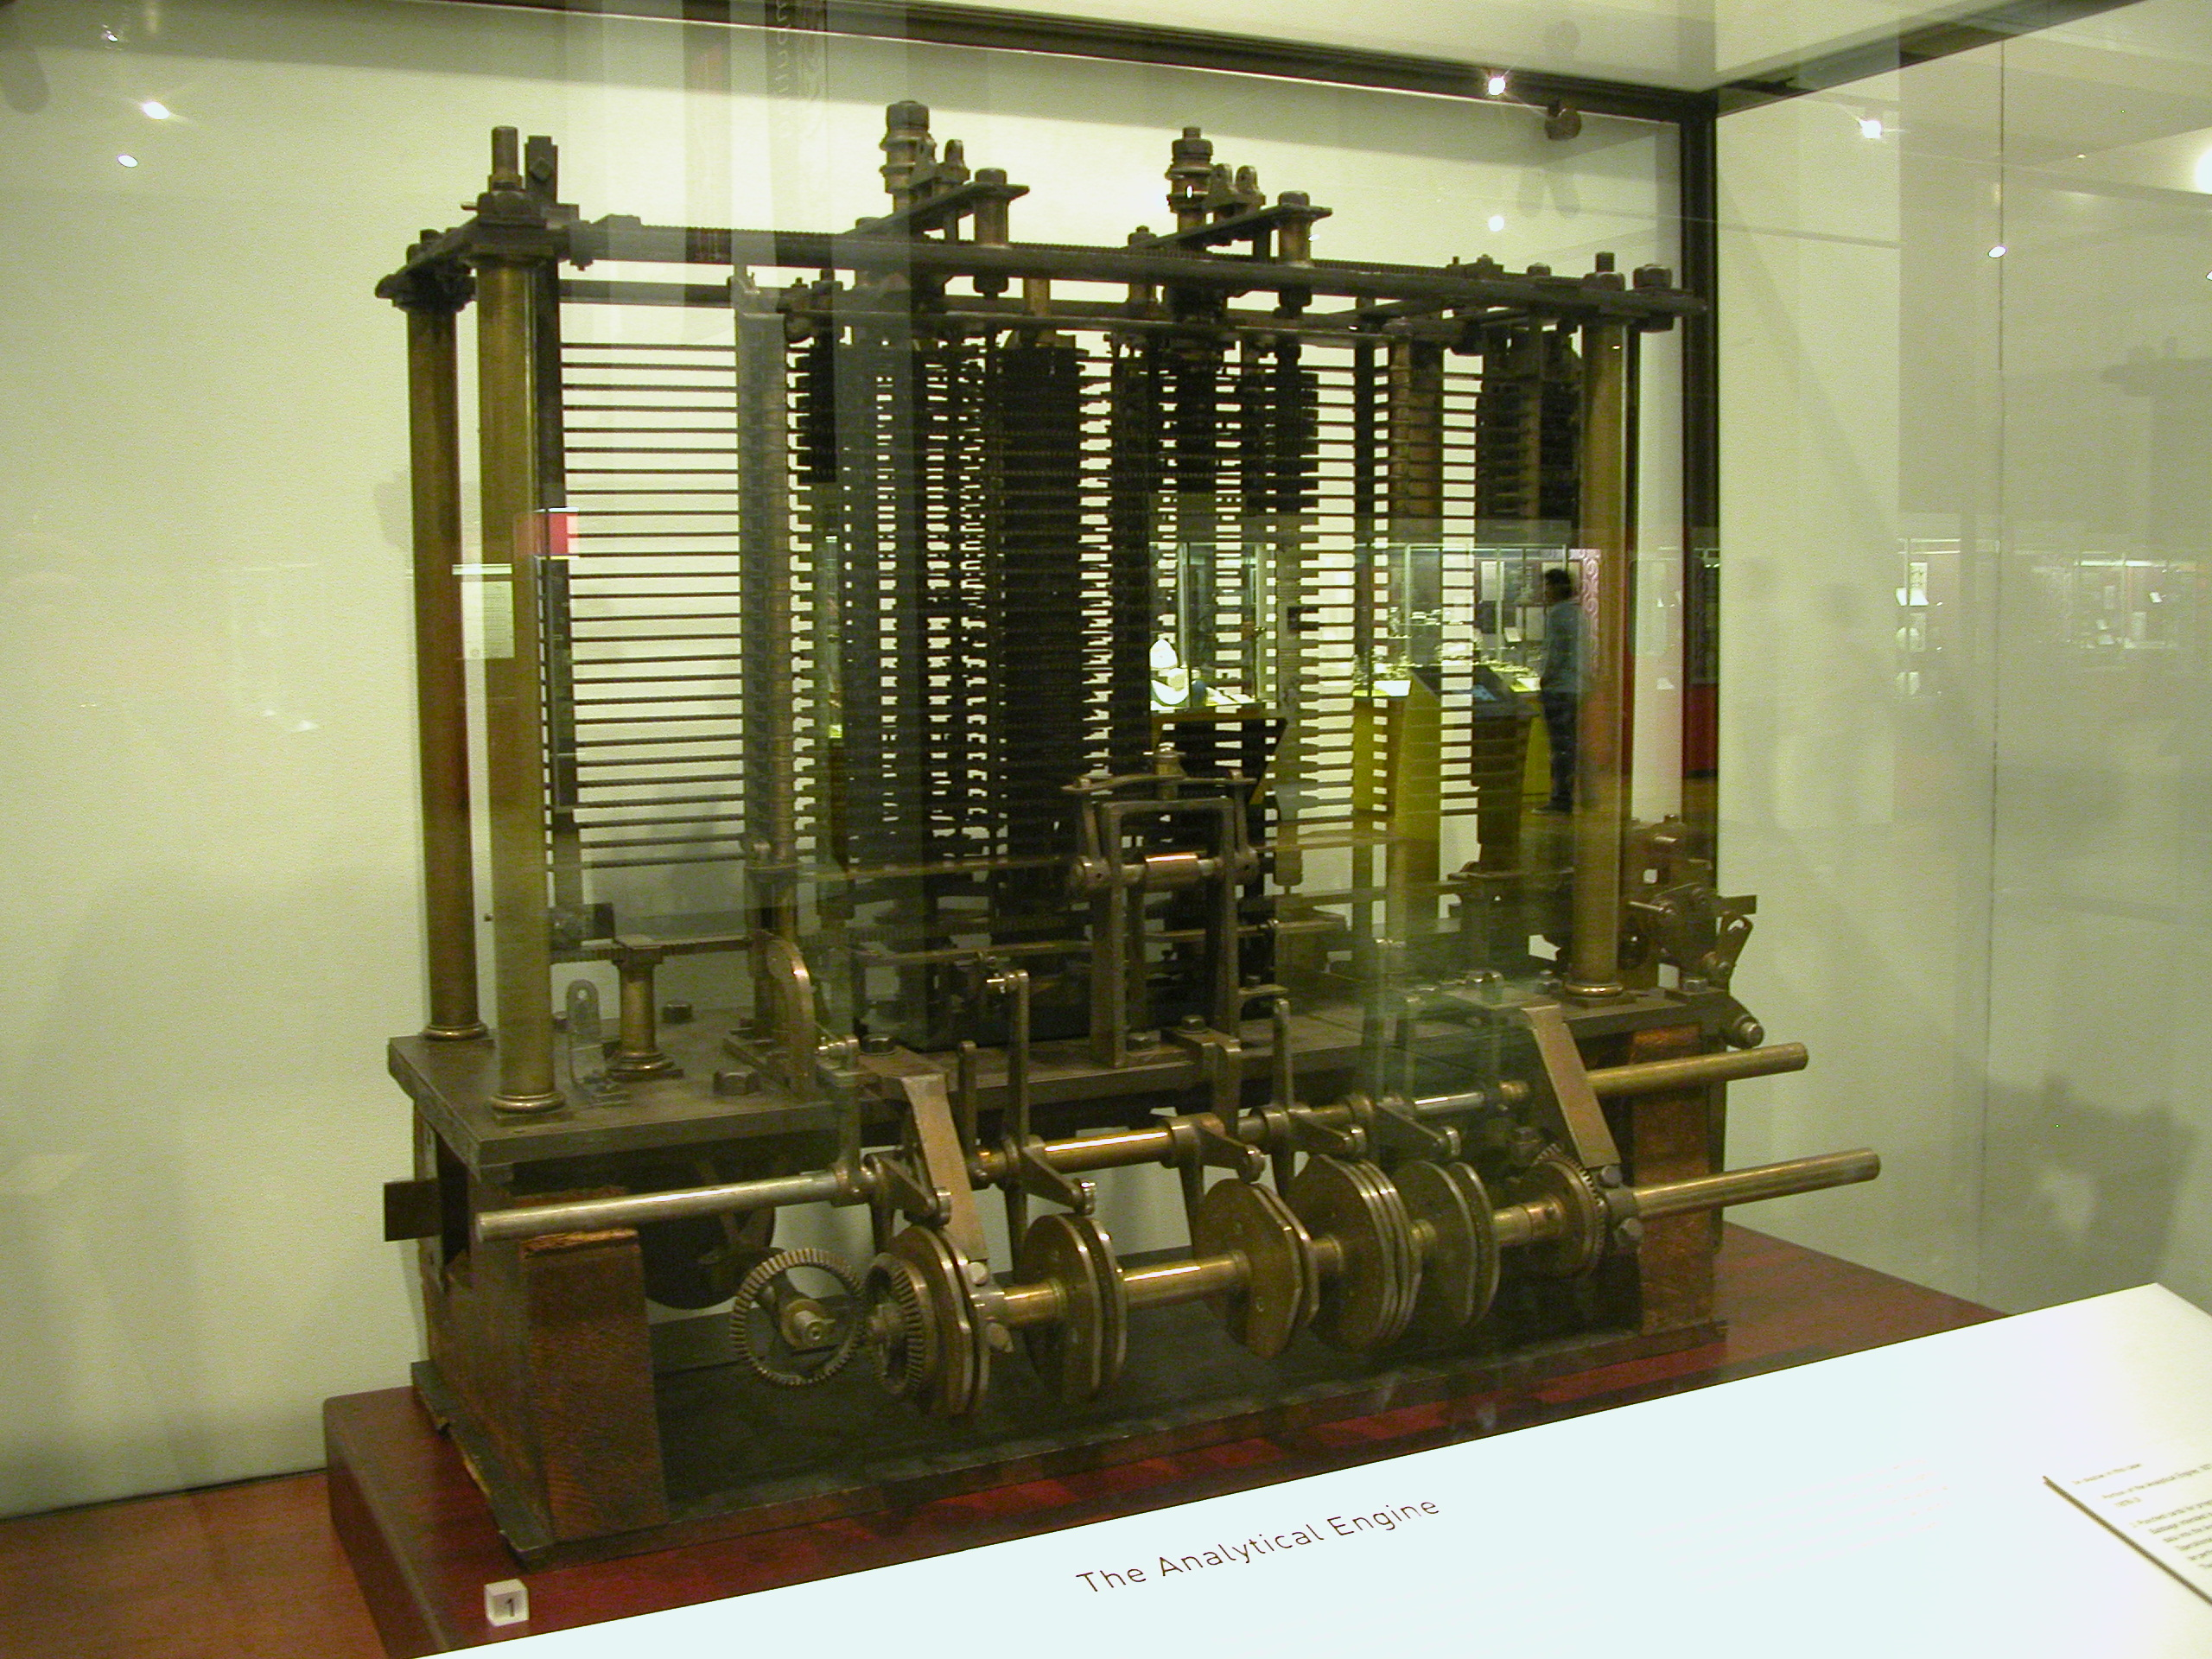
\includegraphics[width=100mm]{imagens/AnalyticalMachine_Babbage_London.jpg}
  \caption[Parte da Máquina Analítica construída por Babbage, cortesia
  Wikipédia]{Parte da Máquina Analítica construída por Babbage, cortesia
  Wikipédia}
  \label{fig:maquina-analitica}
\end{center}
\end{figure}

Nesse contexto, insere-se Ada Lovelace, filha do poeta Lord Byron, considerada a
primeira programadora da humanidade. Ada concebeu diversos conceitos importantes
que vão desde a ideia de subrotina, passando por laços de repetição até o
conceito de desvios condicionais.

Em 1703 Gottfried Leibniz desenvolveu a lógica em um sentido formal e matemático,
fazendo uso do sistema binário. Posteriormente, George Boole, em 1854 publicou
seu trabalho sobre a álgebra e lógica booleana, com valores expressos apenas em
termos de 0 (falso) ou 1 (verdadeiro)

Avançando para 1890, Herman Hollerith inventou uma máquina capaz de
processar dados baseada na separação de cartões perfurados. Seu invento foi
utilizado no censo demográfico desse mesmo ano, diminuindo o tempo para o
processamento dos dados de 7,5 anos para 2,5 anos. Posteriormente, em 1924,
Hollerith fundou uma empresa para fabricar máquinas de tabulação, a
International Business Machines, atualmente IBM, uma gigante do ramo de
informática, que perdura até hoje.

\section{De 1900 aos dias atuais}
Diversas tecnologias agora usadas para propósitos civis surgiram para suprir uma
demanda militar. Dentro da computação não foi diferente. A Segunda Guerra
Mundial foi responsável por diversos avanços na área, sendo um de seus expoentes
a criação do \emph{Eletronic Numerical Integrator and Computer}, o ENIAC I em
1946 para o cálculo de tragetórias balísticas. O ENIAC I era um computador
totalmente elétrico, diferentemente de seus concorrentes eletromecânicos, que
atingia a marca de 500 multiplicações por segundo. \cite{introducao-ilustrada-computacao}

A operação de tal computador era muito complexa pois um programa era feito
rearranjando a fiação em um painel. A partir desse momento, John Von Neumann,
matemático húngaro, propôs o que seria posteriormente conhecido como a
arquitetura de von Neumann: Um computador seria composto por quatro partes: Uma
unidade de memória, onde seriam armazenadas as instruções do(s) programa(s)
carregado(s), uma unidade lógico-artimética, responsável pelo cálculo das
operações, uma unidade de entrada e saída para o computador comunicar-se com o
mundo externo e uma unidade de controle que orquestraria esses componentes. Tal
arquitetura, baseada no cérebro humano fez com que computadores fossem chamados
também de ``Cérebros eletrônicos''.\cite{wiki:historia-computacao}

Outra revolução surgiu na Universidade de Stanford em 1946 quando o transistor
foi criado. Menor, mais barato e mais eficiente que as válvulas, permitiu a
computação dar um salto, com um crescimento exponencial na complexidade e
velocidade dos sistemas enquanto diminuia custos. Esse comportamento
posteriormente ficou conhecido com a Lei de Moore que diz: ``O número de
transistores dos chips dobra a cada 18 meses.''. Realmente tal profecia
concretizou-se, com a existência de circuitos de grande
escala de integração (VLSI, em inglês) com mais de $10^9$ transistores em uma
área comparável ao de uma unha.

%\usepackage{graphics} is needed for \includegraphics
\begin{figure}[htp]
\begin{center}
  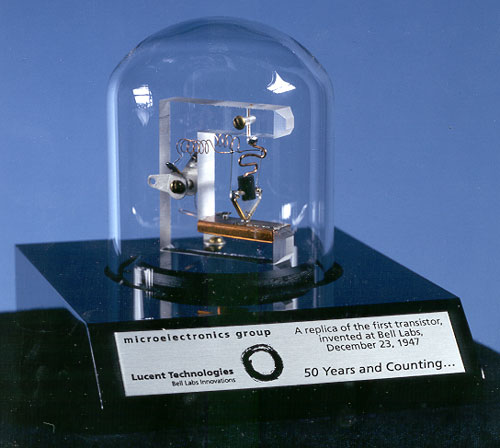
\includegraphics[width=100mm]{imagens/Replica-of-first-transistor.jpg}
  \caption[Réplica do primeiro transistor funcional, cortesia Wikipédia]{Réplica
  do primeiro transistor funcional, cortesia Wikipédia}
  \label{fig:transistor}
\end{center}
\end{figure}

No campo da Teoria da Computação, o expoente foi Alan Turing e Alonzo Church,
responsáveis por importantes estudos nas áreas da computabilidade. Turing criou
a Máquina de Turing, um dispositivo teórico que através de uma fita
infinitamente longa e uma cabeça de leitura é capaz de calcular tudo que possa
ser computável. Além disso, foi o responsável por ter quebrado a criptografia da
máquina nazista Enigma, por fim, criou o teste de Turing para analisar a
capacidade de uma máquina de apresentar inteligência artificial.

Dos gigantescos Mainframes, caros e desengonçados, a computação foi evoluindo
para um modelo de computadores menores e pessoais, o primeiro exemplo disso foi
o Altair 8800, custava cerca de 400 doláres e se comunicava com o usuário
através de luzes que piscavam. Bill Gates e Paul Allen, então calouros da
Universidade de Harvard, tiveram contato com esse aparelho, construindo uma
versão da linguagem Basic para ela. Posteriormente a dupla viria a se reunir
para formar mais uma gigante da informática, a Microsoft.

Paralelamente, em 1976, Steve Jobs e Steve Wozniak juntaram-se para vender um
computador projetado por Wozniak, nascia nesse momento a Apple e seu primeiro
produto o Apple I. Com um investimento da Intel e ideias de interfaces
(gráficas) colhidas do Xerox Parc a empresa criou o primeiro computador pessoal
de sucesso, o Apple II. Por certo tempo, a Apple permaneceu dominante no mercado
de computadores pessoais, sendo desbancada somente com a vinda do IBM-PC.

Os IBM-PCs e versões compatíveis apontaram para o avanço do uso do computador
como ferramenta de uso profissional, não mais apenas um hobby de jovens
entusiastas. Contudo, a IBM não possuía um Sistema Operacional (SO). Nesse
momento, surge novamente a Microsoft oferecendo um SO (que na realidade foi
comprado de outra empresa) com a condição que ela mantenha os direitos
intelectuais e possa distribuir versões modificadas. Os executivos da IBM, com a
crença de que o verdadeiro valor dos computadore estava no hardware e não no
software, aceitaram, atitude essa que pavimentou o caminho para que a Microsoft
se tornasse uma das mais poderosas empresas de informática do mundo, e Bill
Gates um bilionário. \cite{wiki:microsoft}

%\usepackage{graphics} is needed for \includegraphics
\begin{figure}[htp]
\begin{center}
  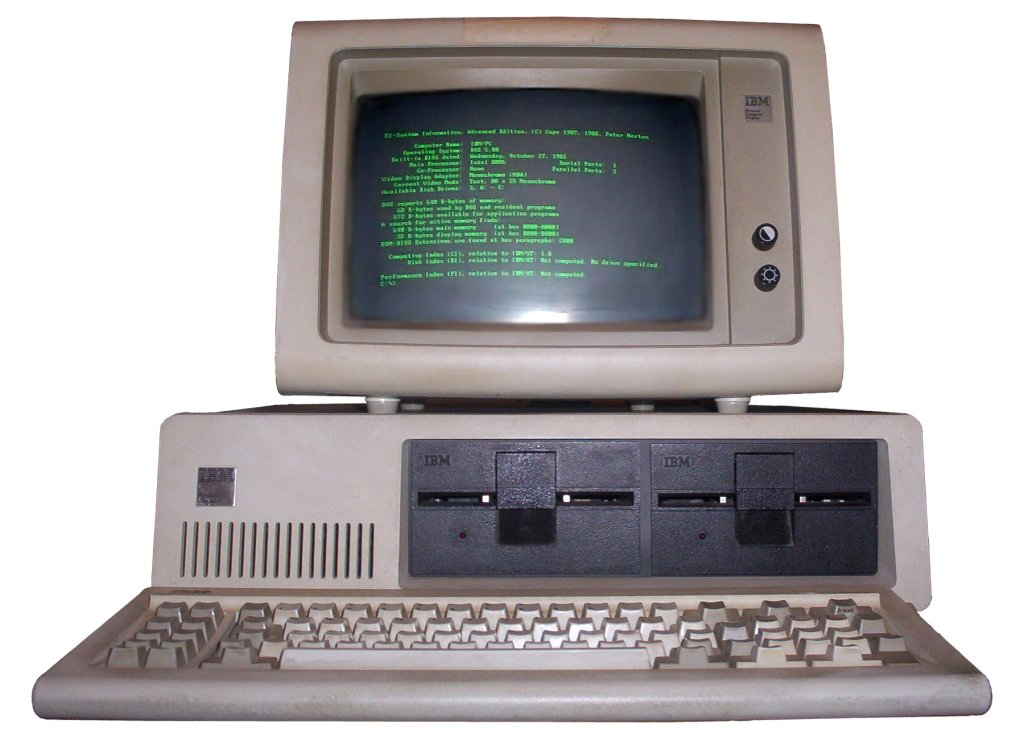
\includegraphics[width=100mm]{imagens/IBM_PC_5150.jpg}
  \caption[O primeiro IBM PC, modelo 5150, cortesia Wikipédia]{O primeiro IBM
  PC, modelo 5150, cortesia Wikipédia}
  \label{fig:ibm-pc}
\end{center}
\end{figure}

Uma das últimas revoluções acontecidas, e assunto do próximo capítulo, foi a
invenção da ARPANET, embrião da Internet atual, em 1975 como uma rede projetada
pelo governo americano durante a Guerra Fria para conectar as bases militares,
departamentos de pesquisa do governo americano e universidades. Sua abertura
comercial viria somente em 1988, já como Internet, com serviços provedores
de correio eletrônico. Mas, a grande explosão da rede viria apenas com o advento
da \emph{World Wide Web} (WWW), criada por Tim Berners-Lee, pesquisador do CERN,
na Europa. 

\chapter{História das redes de computadores}
\section{Telecomunicações analógicas}
Algumas invenções, como o uso de sinais de fumaça por índios ou o de semáforos,
comuns na Idade Média são consideeradas os primórdios da comunicação à
distância. Porém, foi o telégrafo, criação de Samuel Morse 1838, a primeira ferramenta para
facilitar a comunicação de dados, fazendo o uso do Código Morse para codificar suas
mensagens a serem transmitidas por cabos telegráficos, inclusive submarinos.

%\usepackage{graphics} is needed for \includegraphics
\begin{figure}[htp]
\begin{center}
  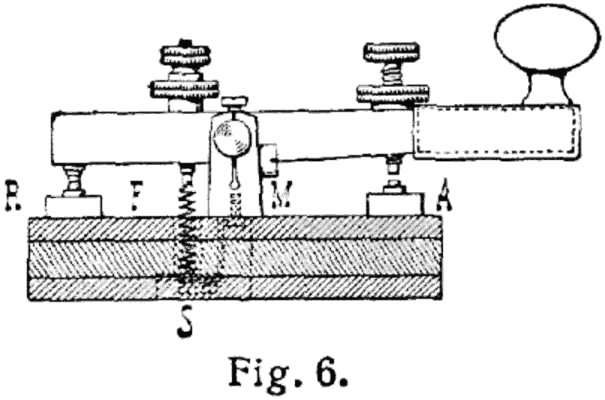
\includegraphics[width=100mm]{imagens/L-Telegraph1.png}
  \caption[Imagem da patente do telégrafo de Morse, cortesia Wikipédia]{Imagem
  da patente do telégrafo de Morse, cortesia Wikipédia}
  \label{fig:telegrafo}
\end{center}
\end{figure}

Em 1876, Alexander Graham Bell patenteou o telefone, com serviços comerciais já
operando em ambos os lados do Atlântico em 1878 e 1879. Depois, a radiotelefonia
aproveitou-se do trabalho de Nikola Tesla e Marconi para permitir comunicações
sem fio.

\section{Telecomunicações digitais e a Guerra}
Mais futuramente, com o avanço da computação e o advento dos ``terminais
burros'' conectados a \emph{mainframes}, houve uma crescente necessidade de
interconexão entre os computadores. No contexto da Guerra Fria, o governo
americano sentiu a necessidade de implementar uma rede de comunicação
descentralizada, capaz de sobreviver mesmo que parte dela seja comprometida por
um ataque (nuclear, por exemplo).

Dessa ideia, surgiu a ARPANET, sob a responsabilidade do Departamento de Defesa
norte-americano, interligando departamentos de pesquisa do governo americano e
universidades. Um de seus avanços foi o uso de comutação de pacotes, tal
arquitetura permite uma maior flexibilidade em relação à comutação de circuito.

Com rápido aumento da ARPANET, com nodos cada vez mais heterogêneos e sem uma
regulamentação extensa, surgiu a necessidade de criação de diversos padrões e
protocolos. O surgimento do TCP/IP em 1974 e do padrão Ethernet foram de suma
importância pois permitiram até hoje a escalabilidade da Internet, independente
da heterogeneidade de certas redes. O TCP/IP, por exemplo, pressupõe a
não-confiabilidade da rede de interconexão, transferindo a responsabilidade da
integridade dos pacotes para os nodos da rede, diferentemente de protocolos
anteriores. \cite{wiki:arpanet}

%\usepackage{graphics} is needed for \includegraphics
\begin{figure}[htp]
\begin{center}
  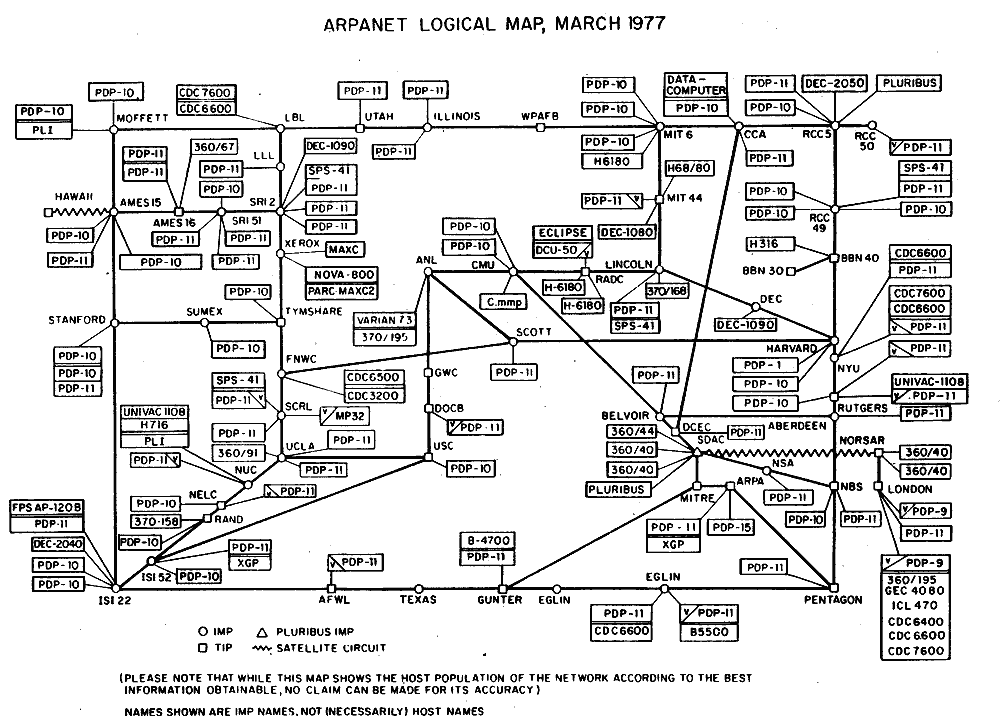
\includegraphics[width=150mm]{imagens/Arpanet_logical_map,_march_1977.png}
  \caption[Mapa da ARPANET em 1977, cortesia Wikipédia]{Mapa da ARPANET em 1977,
  cortesia Wikipédia}
  \label{fig:arpanet}
\end{center}
\end{figure}

Outro avanço importante foi a criação do modelo OSI (\emph{Open Systems
Interconnection}) que é responsável por estabelecer várias camadas com
responsabilidades diversas em uma rede de computadores, estabelecendo, também,
protocolos para essas.

Com o crescimento da rede, gerenciar listas de todos os nodos conectados
foi tornando-se mais complicado. Frente à essa demanda, em 1980
\cite{historia-redes-gdh} surgiu o sistema de nomes de domínio (DNS),
responsável por traduzir endereços IP para nomes legíveis e mais facimente
memorizávies por humanos.

\section{A Internet e a WWW}
Com a vinda do TCP/IP, foi possível interconectar qualquer rede, não importando
suas características. Isso possibilitou a comunicação ``entre redes'' ou
\emph{internet}, como pode ser percebido na primeira menção à rede mundial de
computadores em uma \emph{Request for Comments} (RFC) redigida por Vinton Cerf,
inventor do TCP/IP e considerado um dos pais da Internet: \emph{RFC 675 -
Specification of Internet Transmission Control Program}. \cite{wiki:history-internet}

Até esse momento, a Internet era composta por aplicações como a Usenet, serviços
de FTP, Gopher, e-mail etc. Porém, sua abrangência se expandiria ainda mais
através do trabalho de Tim Berners-Lee, pesquisador do CERN, que aproveitando-se
da noção do \emph{hipertexto}, criou a \emph{World Wide Web}, baseada no uso do
protocolo HTTP, da linguagem de marcação HTML e dos identificadores únicos
(URIs). Seu trabalho flexibilizou e facilitou a criação e consumo de conteúdo,
sendo a maneira mais usada para acessar-se a Internet atualmente.

Com o crescimento exponencial da Internet e da WWW, houve a necessidade de
facilitar a busca por conteúdo na rede de computadores. Essa demanda veio a ser
suprida com o advento de mecanismos de busca, que varrem as páginas web em busca
de conteúdo novo, catalogam e permitem sua busca. Os primeiros nessa área
foram o AltaVista e o Yahoo!, que posteriormente foram desbancados por um novo
concorrente, o Google, que emprega algoritimos sofisticados, analisando centenas
de fatores diferentes para fornecer o melhor conteúdo a seus usuários.

\section{Últimos avanços}
Na década dos anos 2000 percebeu-se a consolidação da Internet na vida das
pessoas. Um exemplo disso, foi o surgimento da Web 2.0, expressão cunhada por
Tim O'Reilly para apresentar uma mudança no paradigma da WWW. Os usuários
passaram a deixar de serem consumidores de conteúdo para participar ativamente
da produção de material. Essa foi a década dos blogs, das redes sociais, dos
podcasts, etc. Um vídeo famoso que aborda essa área é o \emph{Web 2.0 ... The Machine
is Us/ing Us } de Michael Wesch. \cite{web20-the-machine-is-us}

Outro avanço na área é a vinda da Computação em Nuvem. Ela pode ser definida com
o uso da capacidade computacional de um parque de servidores sob demanda através
da Internet, de maneira similar ao sistema de distribuição elétrica. Favoráveis 
dessa tecnologia argumentam que isso é uma maneira de remover a complexidade da
manutenção do sistema de usuários finais e empresas, reduzindo custos e
facilitando uso. Já os desfavoráveis dizem que os riscos à privacidade
envolvidos em fornecer dados sigilosos a terceiros ultrapassam as vantagens.
\cite{wiki:computacao-nuvem}

Ainda, com a demanda de cada vez maior velocidade e o iminente
esgotamento da capacidade de expansão da velocidade usando fios de cobre, há
pesquisas em andamento para estudar as redes de fibra ótica, que já atingem 10
Gbps e com possibilidade de aumentar-se esse valor em uma ou mais ordens de
grandeza.

Atualmente devido ao grande sucesso da Internet, o número de endereços de IP
disponível para ser registrado está chegando ao fim, o esgotamento do espaço de
endereçamento IPv4 deve acontecer entre 2010 e 2011. Desse modo, esforços estão
sendo concentrados para o desevolvimento e adoção da nova versão do protocolo
IP, o IPv6, que permite aproximadamente $2^{128}$ endereços distintos. Isso é
parte importante do caminho para um futuro onde acredita-se que tudo estará
conectado à Internet, a Internet das Coisas, dentro da ideia de Computação
Ubíqua. Roupas, objetos domésticos, carros, tudo possuirá sensores sem fio e estará
conectado à rede, transmitindo e recebendo informações.

%\usepackage{graphics} is needed for \includegraphics
\begin{figure}[htp]
\begin{center}
  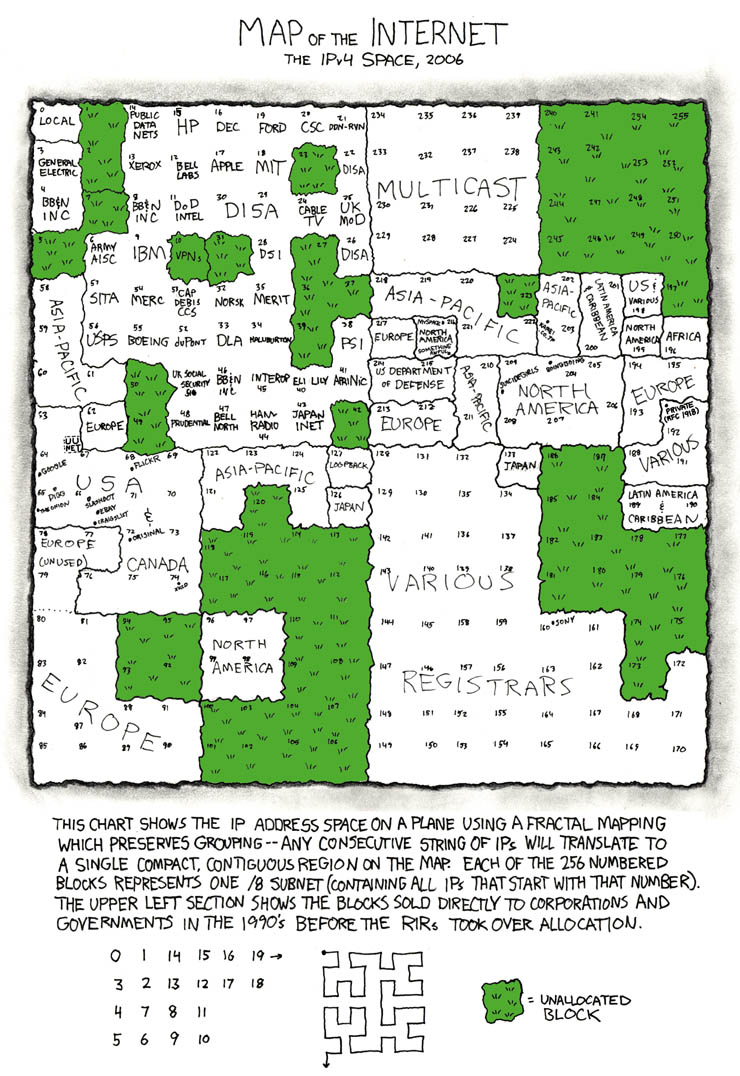
\includegraphics[width=150mm]{imagens/map_of_the_internet.jpg}
  \caption[Mapa da Internet em 2006, cortesia do blog xkcd]{Mapa da Internet em 2006, cortesia do blog xkcd}
  \label{fig:map-intenet}
\end{center}
\end{figure}

\bibliographystyle{abnt-alf}
\bibliography{referencias}
\end{document}